\documentclass[11pt,oneside,a4paper]{article}

% Packages
\usepackage{cite}
\usepackage{graphicx}
\usepackage{subfigure}
\usepackage{float}
\usepackage{url}

\begin{document}

% paper title
% can use linebreaks \\ within to get better formatting as desired
\title{Probabilistic Robotics Lab 1 \\ Introduction to Turtlebot}
%
%
% author names and IEEE memberships
% note positions of commas and nonbreaking spaces ( ~ ) LaTeX will not break
% a structure at a ~ so this keeps an author's name from being broken across
% two lines.
\author{Rodrigo~Caye~Daudt}


% The paper headers
\markboth{Lab 1}%
{Introduction to Turtlebot}


% make the title area
\maketitle




% Note that keywords are not normally used for peerreview papers.
%\begin{IEEEkeywords}
%IEEEtran, journal, \LaTeX, paper, template. ln505
%\end{IEEEkeywords}



%%%%%%%%%%%%%%%%%%%%%%%%%%%%%%%%%%%%%%%%%%%%%%%%%%%%%%%%%%%%%%%%%%%%%%%%%%%%%%%
\section{Introduction}

%\IEEEPARstart{T}{his} 
This report describes the work done for lab 1 assignment for the Probabilistic Robotics class. The main objectives of this assignment were to learn how to connect and send commands to the turtlebots, generate maps for navigation automatically, and to program a python script to control the turtlebot's movement.

%%%%%%%%%%%%%%%%%%%%%%%%%%%%%%%%%%%%%%%%%%%%%%%%%%%%%%%%%%%%%%%%%%%%%%%%%%%%%%%
\section{Connexion to turtlebots and Gazebo simulator}

The first part of this lab consisted on configuring the computers to connect to the turtlebots. In the two hours available, it was possible to connect to the turtlebot and use the teleoperation node, but we didn't achieve the mapping or drive to goal tasks on the lab robots.

To accomplish the remaining tasks the computer was reconfigured to run all the operations locally on a simulated turtlebot using the Gazebo simulator. This simulator provides a physical model of the turtlebot with all its working components and can be used for simulations of the turtlebot in many different settings. On the simulator the SLAM node was tested and the "drive to goal" controller was developed.

%%%%%%%%%%%%%%%%%%%%%%%%%%%%%%%%%%%%%%%%%%%%%%%%%%%%%%%%%%%%%%%%%%%%%%%%%%%%%%%
\section{Teleoperation, mapping, and navigation}

The first task was to control the movement of the turtlebot using teleoperation from the computer's keyboard. This was achieved using a standard turtlebot package called \textit{turtlebot\_teleop keyboard\_teleop.launch}. This allowed us to move the turtlebot (real or simulated) as desired, which was useful for the mapping step.

Once we had control over the turtlebot's movement, our next task was to generate a small map of the environment where the robot was located. Using the node \textit{turtlebot\_navigation gmapping\_demo.launch} in conjunction with the teleoperation node we were able to create a map of a small section of the environment. This map was visualised in real time on RViz running on the node \textit{turtlebot\_rviz\_launchers view\_navigation.launch}. An image captured during the process of building the map can be seen in Fig. \ref{map1}.

Once a map had been generated and saved, we used the node \textit{turtlebot\_navigation amcl\_demo.launch} to navigate the map automatically to a chosen goal. Using RViz we were able to select a point on the map as the goal for the turtlebot, and its trajectory was automatically calculated. Figures \ref{goal1}-\ref{goal3} show three different stages of the turtlebot on its way to the goal. The behaviour of the turtlebot during this process was somewhat erratic, but it reached the goal without any problems.

\begin{figure}
	\centering
	\subfigure[RViz visualisation of map generated by \textit{slam\_gmapping} node]{\label{map1}
		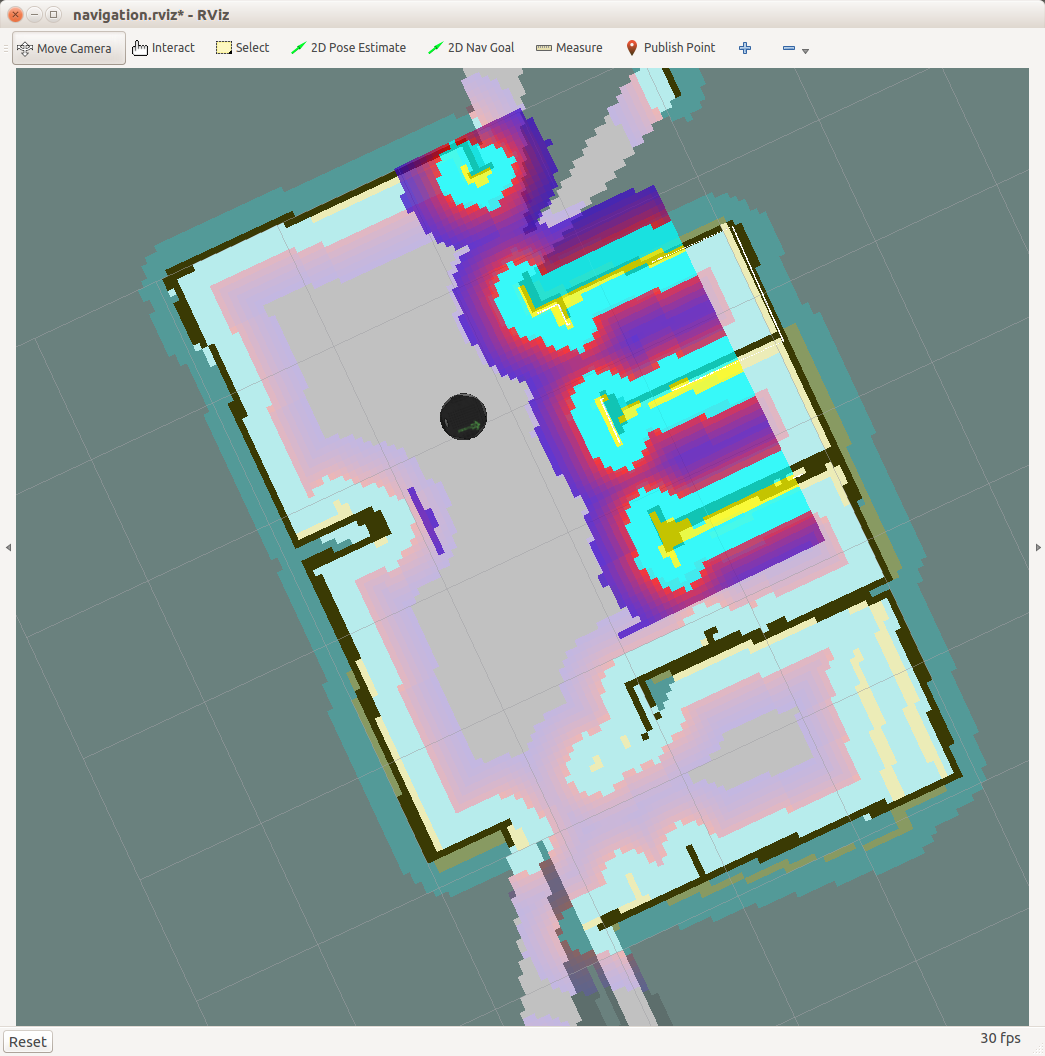
\includegraphics[width=2in]{figures/map1.png}}~
	\subfigure[Beginning of navigation]{\label{goal1}
		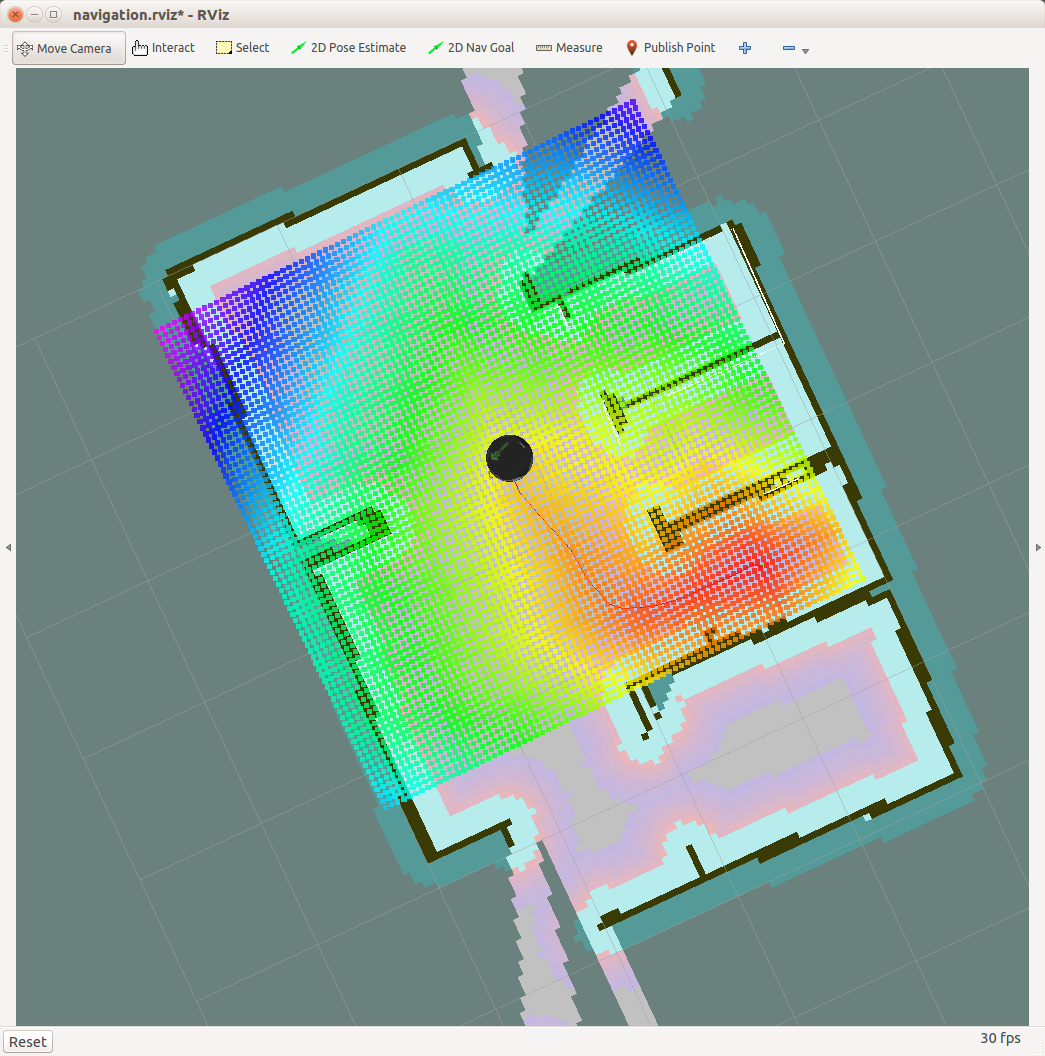
\includegraphics[width=2in]{figures/goal1.png}}\\
	\subfigure[Middle of navigation]{\label{goal2}
		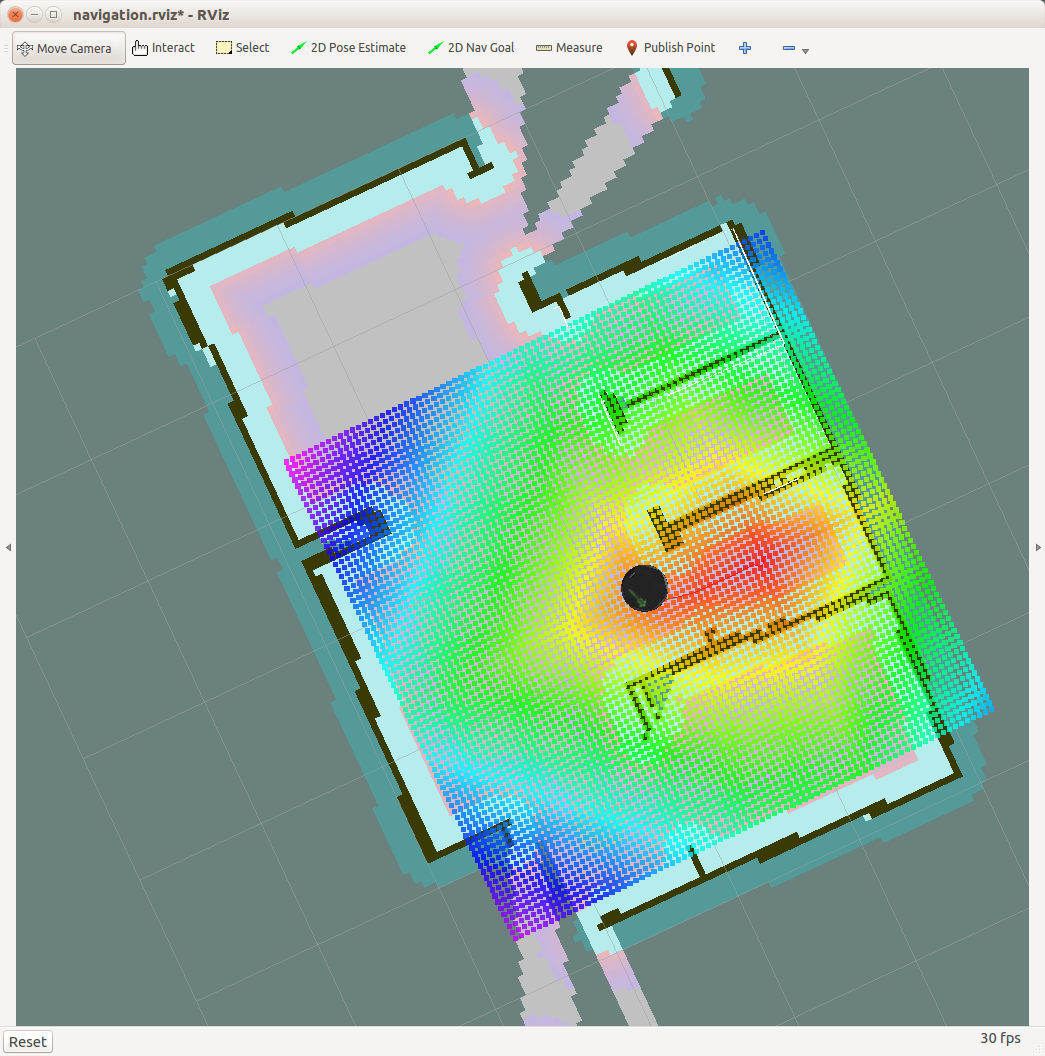
\includegraphics[width=2in]{figures/goal2.png}}~
	\subfigure[End of navigation]{\label{goal3}
		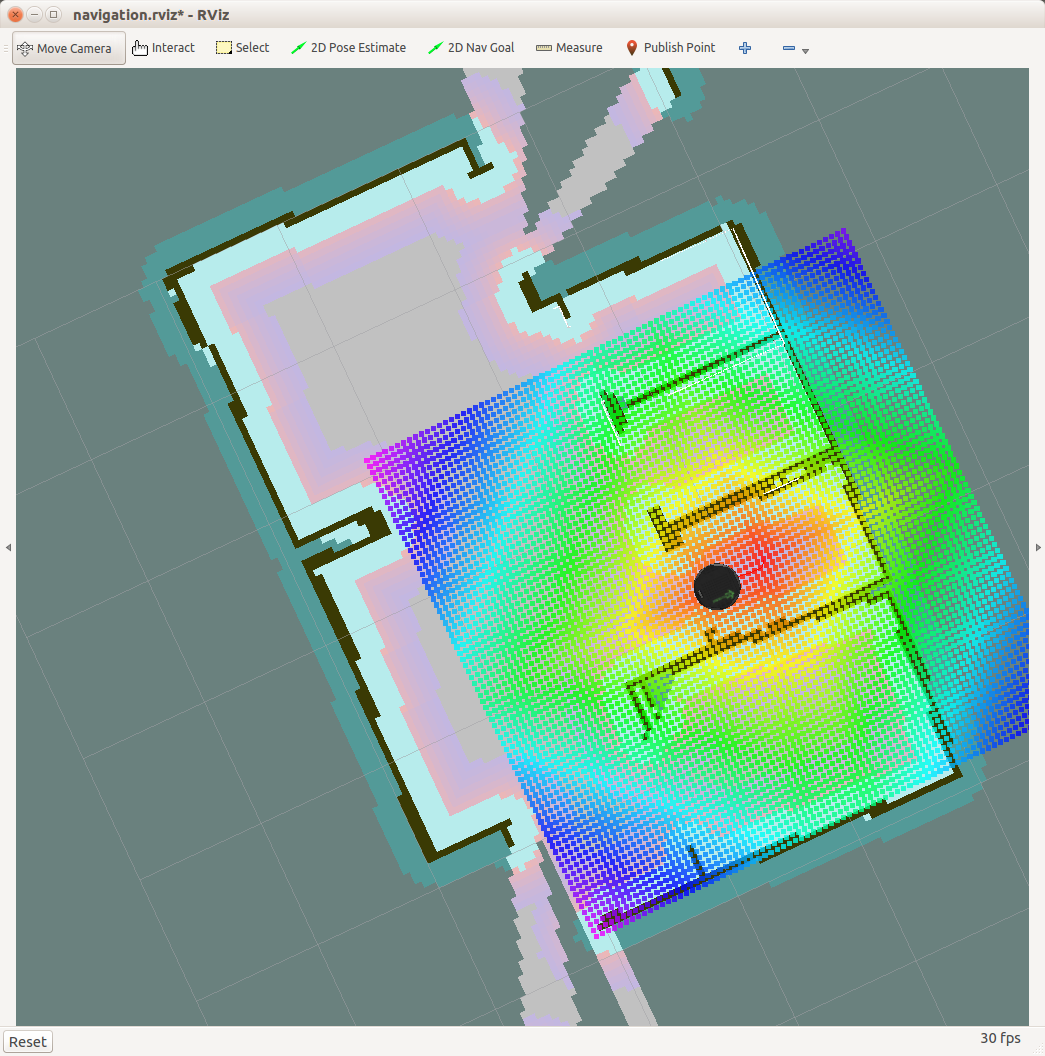
\includegraphics[width=2in]{figures/goal3.png}}
	\caption{Movement of turtlebot towards desired goal controlled by \textit{turtlebot\_navigation}}
	\label{goals}
\end{figure}

%%%%%%%%%%%%%%%%%%%%%%%%%%%%%%%%%%%%%%%%%%%%%%%%%%%%%%%%%%%%%%%%%%%%%%%%%%%%%%%
\section{Turtlebot driver}

The next task was to program a node to control the movement of the turtlebot to move it towards a goal. This can be divided in two main parts: the communication to the turtlebot, and the calculation of the control signals.

Two topics were essential in this operation. The first one was \textit{/odom}, whose messages contain information about the turtlebot's position and orientation. The messages published on this node are of type \textit{nav\_msgs/Odometry}. A conversion from quaternion orientation was needed for our calculations, and this transformation was done using \textit{tf.transformations.euler\_from\_quaternion}. The other relevant topic was \textit{/cmd\_vel\_mux/input/navi}, which was used to send messages of type \textit{geometry\_msgs/Twist} to the turtlebot containing the desired linear and angular velocities.

The velocity signals were calculated using a PD controller with some extra non-linear additions. This provided us with a simple and robust solution that could take the robot to any desired goal as long as no objects were on the way. The robot would first go to the desired coordinates, and after it arrived it would turn to the desired orientation. The non-linear additions to the operations served the purpose of decreasing the time the turtlebot took to reach the goal and to improve its stability. For example, the control signals were clipped at some maximum values to avoid unexpected behaviour or the robot, since it was observed that the robot would behave very strangely for large control signals.

%%%%%%%%%%%%%%%%%%%%%%%%%%%%%%%%%%%%%%%%%%%%%%%%%%%%%%%%%%%%%%%%%%%%%%%%%%%%%%%
\section{Difficulties during development}

Many configuration and networking issues were faced during the development of this project. Also, at first it was not clear that the reason that the turtlebot was behaving strangely was the large control signals that were being sent. This led to suspecting something was wrong with the code logic, since it was not expected to see the robot spinning indefinitely after a short strong signal was applied. Finally, the documentation for ROS is not very helpful in many cases.


%%%%%%%%%%%%%%%%%%%%%%%%%%%%%%%%%%%%%%%%%%%%%%%%%%%%%%%%%%%%%%%%%%%%%%%%%%%%%%%
\section{Conclusion}

In this session we understood the basics of how to control the turtlebot using ROS. The system was tested with a real turtlebot and with a simulated one using Gazebo. Many turtlebot packages were used to achieve teleoperation, mapping and automatic navigation. A ROS package was developed to guide the turtlebot to a list of chosen goals.




%\begin{figure}
%	\centering
%	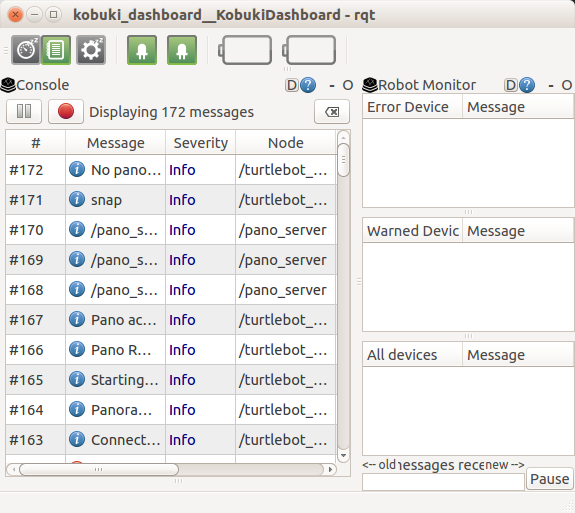
\includegraphics[width=2.5in]{figures/dashboard.png}
%	\caption{Turtlebot dashboard}
%	\label{dashboard}
%\end{figure}

\begin{figure}
	\centering
	\subfigure[rosgraph when performing SLAM]{\label{fig:gmapping}
	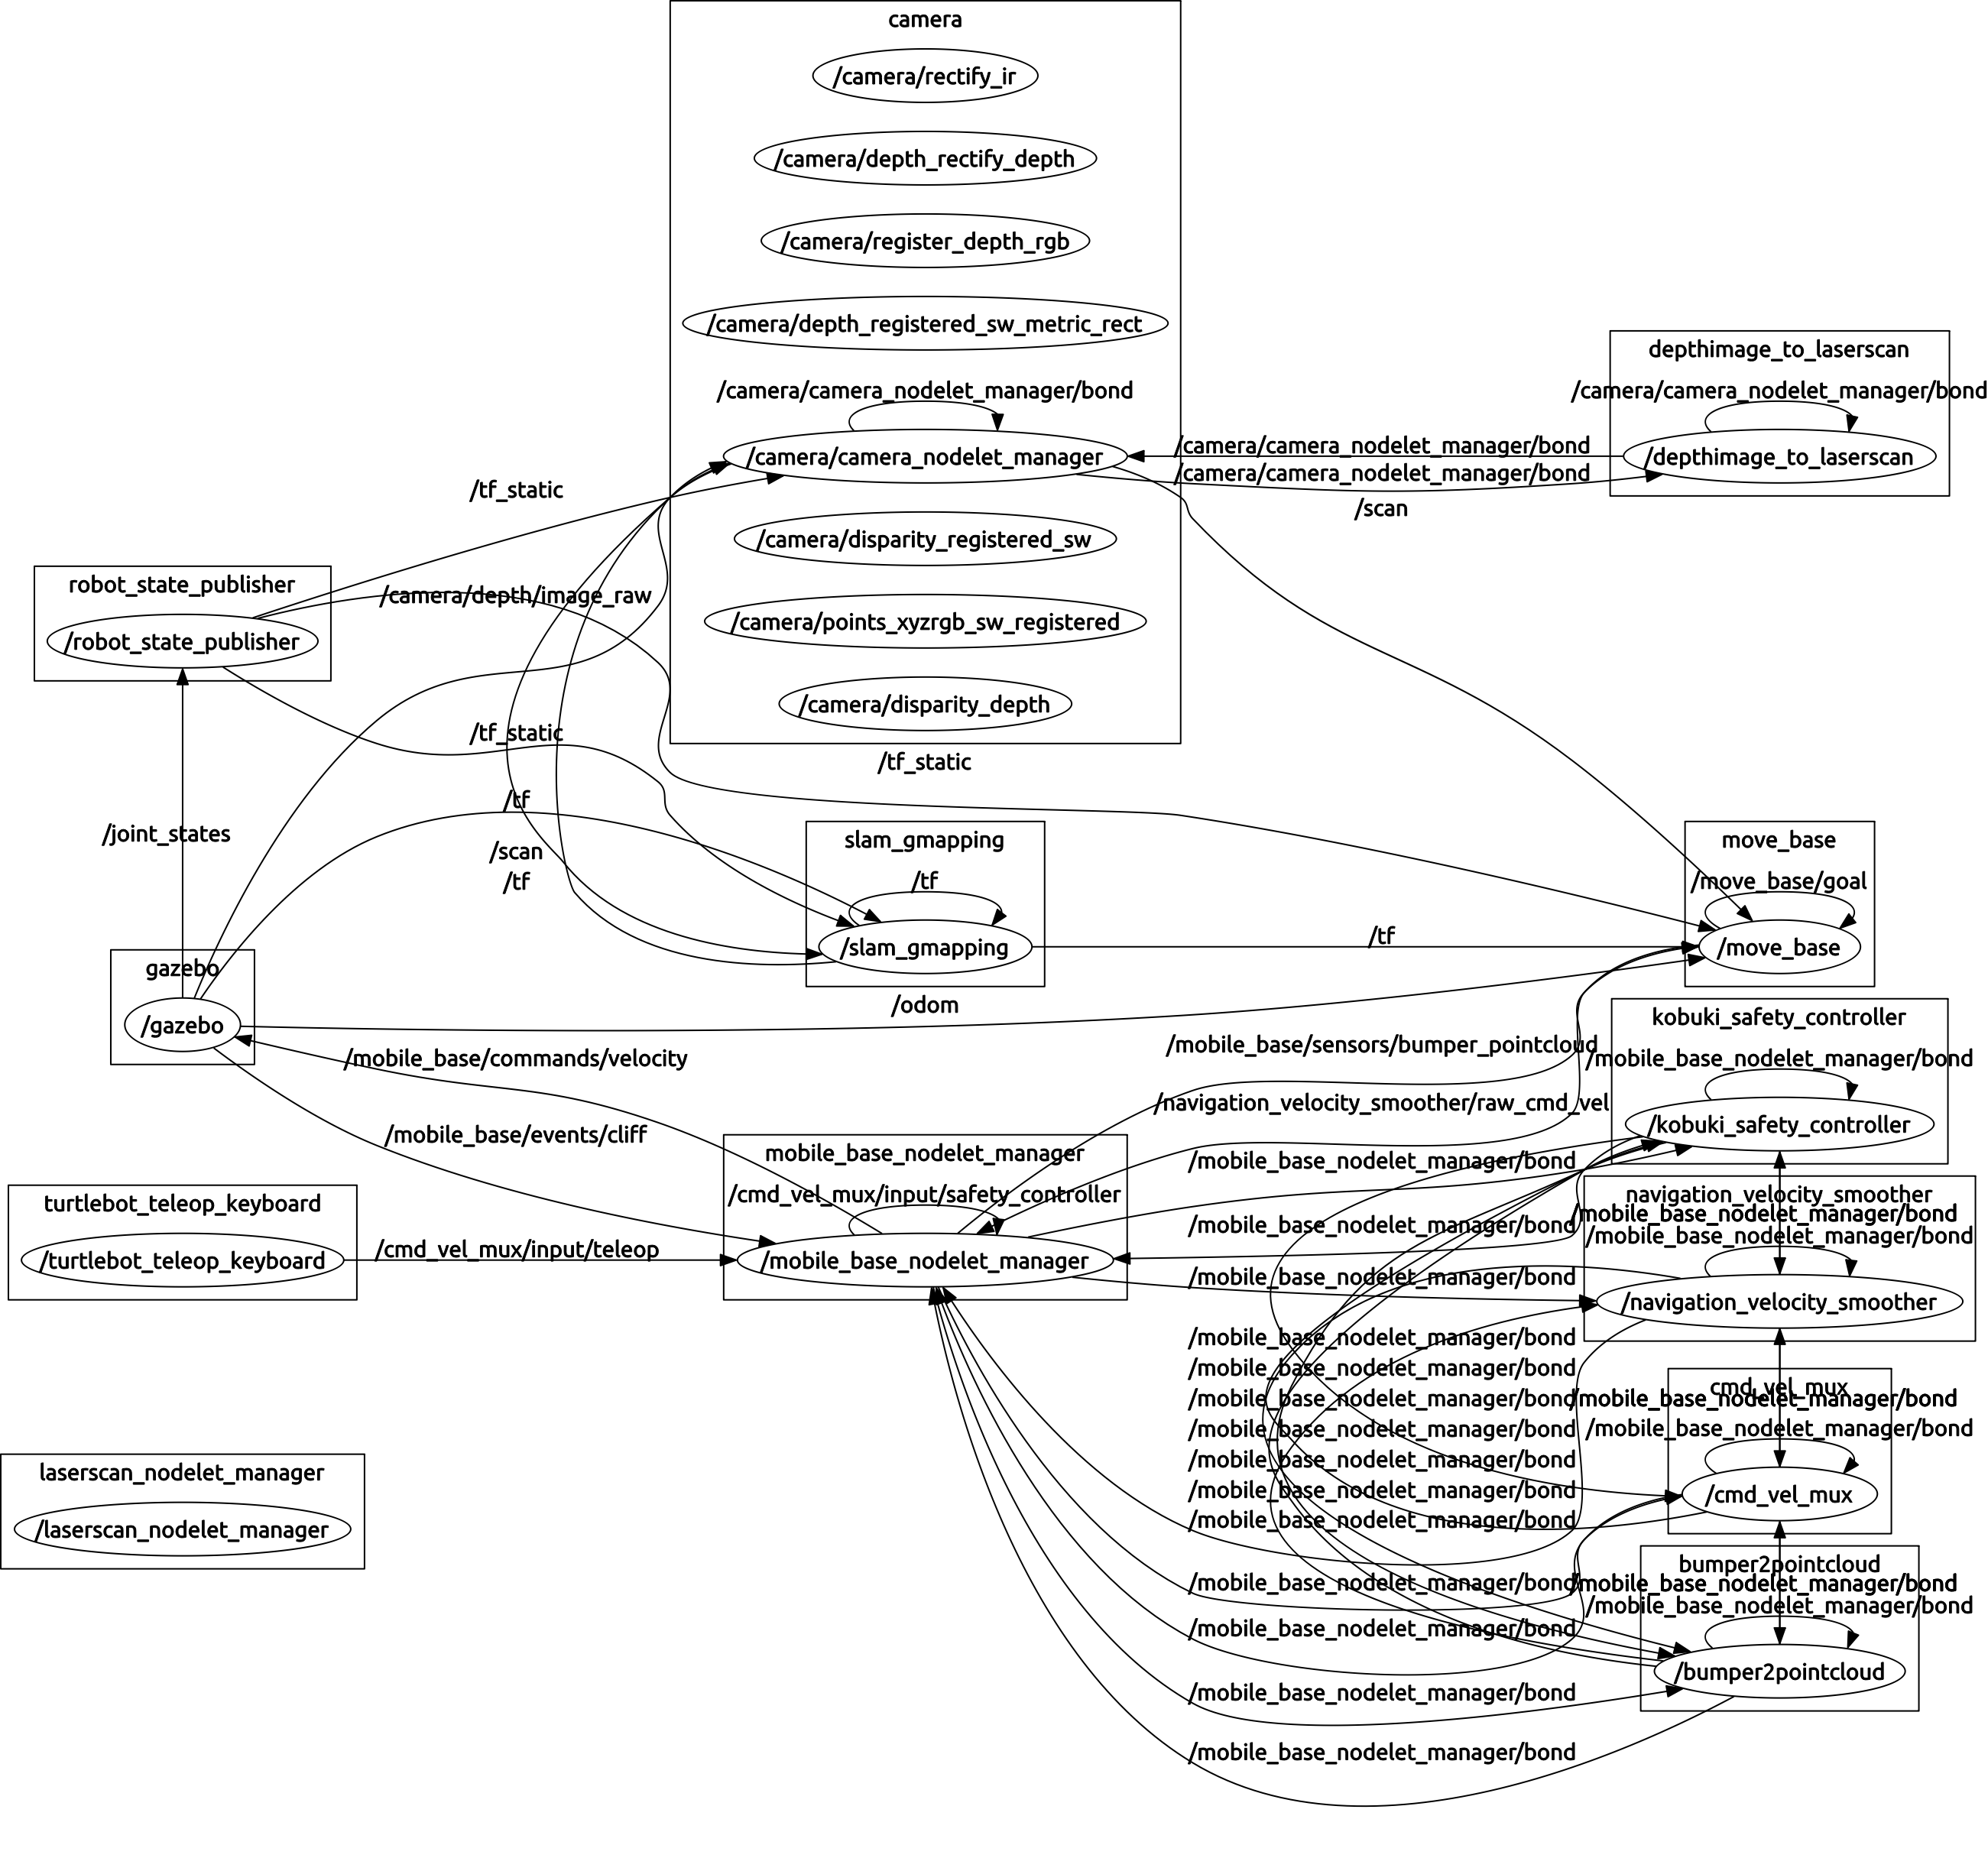
\includegraphics[width=4.9in]{figures/rosgraph_gmapping.png}}\\
	\subfigure[rosgraph when driving to goal]{\label{fig:drive}
	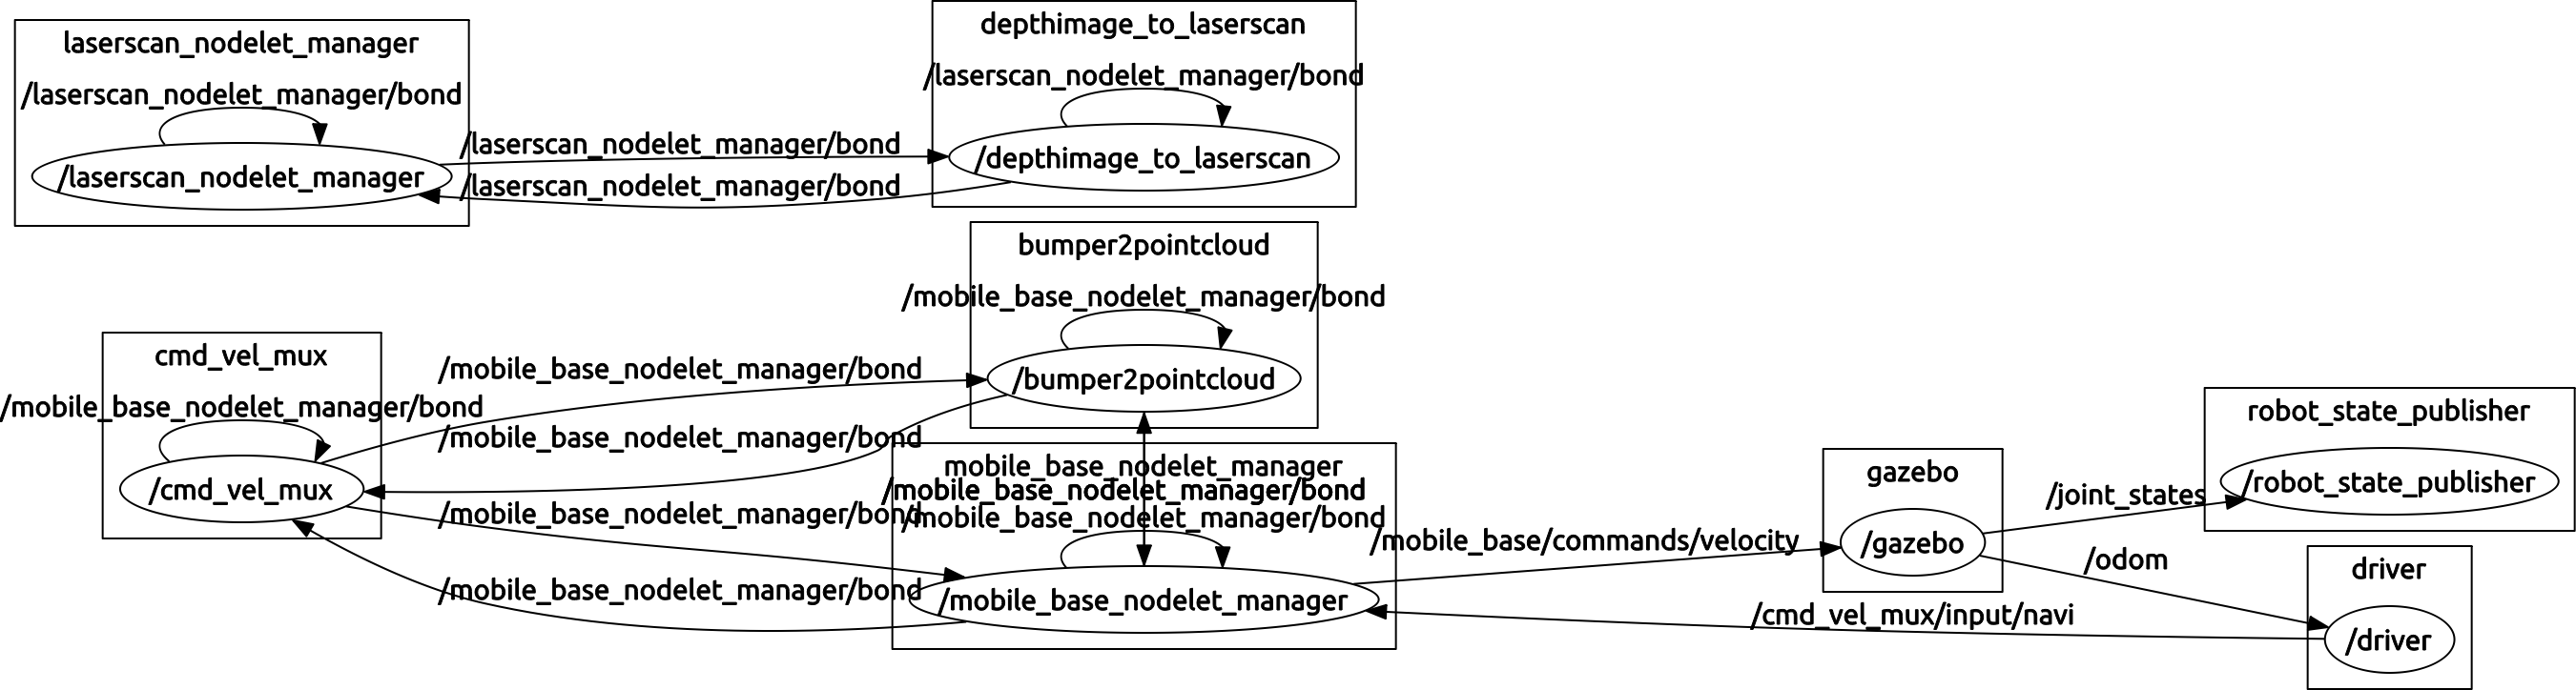
\includegraphics[width=4.9in]{figures/rosgraph_drive.png}}
	\caption{Graphs obtained using rqt\_graph}
	\label{graphs}
\end{figure}







%\appendices
%\section{Proof of the First Zonklar Equation}
%Appendix one text goes here.
%
%\section{}
%Appendix two text goes here.


% use section* for acknowledgement
%\section*{Acknowledgment}
%The authors would like to thank...


%\bibliographystyle{IEEEtran}
%\bibliography{Template_Daudt}


\end{document}


